
Si vuole realizzare una base di dati per un servizio che permette di affittare e prenotare
alloggi di vario tipo ad esempio interi appartamenti, stanze private (camera privata e spazi
comuni) e stanze condivise (spazio in comune e camera condivisa).\newline
Gli utenti si registrano al servizio fornendo indirizzo email, password, nome, cognome,
numero o numeri di telefono. Se l’utente fornisce la foto della carta d’identità, viene
riconosciuto come verificato. Inoltre, l’utente deve indicare un metodo di pagamento per
poter prenotare. Gli utenti possono essere ospiti o “host” ovvero possono a loro volta
ospitare altri utenti del servizio in uno o più alloggi di loro proprietà. Inoltre gli “host” possono
diventare “superhost” se soddisfano i seguenti requisiti:
\begin{itemize}
    \item Devono aver completato almeno 10 soggiorni, per un totale di almeno 100 notti.
    \item Devono aver conservato un tasso di cancellazione dell'1\% (una cancellazione ogni
    100 prenotazioni) massimo.
    \item Devono aver mantenuto una valutazione complessiva di 4,8 \newline considerando tutti i
    soggiorni in tutte le case di sua proprietà.
\end{itemize}
Gli utenti superhost ricevono un badge sul loro profilo.
\newline
\newline
Gli alloggi sono descritti indicando un nome, l’indirizzo (visibile all’ospite solo quando la
prenotazione è confermata, altrimenti è visibile solo il comune), una descrizione, il prezzo per
notte per persona e i costi di pulizia, delle foto, i servizi (ad esempio, cucina, wi-fi, lavatrice,
ecc.), numero di letti e orario di check-in e check-out oltre all’host a cui appartiene, il rating
medio e il numero di recensioni (vedere Fig. 1).
\newline
\newline
Gli utenti possono aggiungere alcune case tra i preferiti. Gli utenti possono avere diverse
liste, ad esempio in base al viaggio che vogliono compiere.
\newline
\newline
Gli utenti possono prenotare degli alloggi di qualsiasi tipo indicando un intervallo di date per il
soggiorno e il numero degli ospiti. Se gli ospiti sono a loro volta utenti del servizio, se ne
possono indicare i nominativi. La prenotazione deve essere confermata o rifiutata dall’host.
La prenotazione ha un costo totale e se confermata viene eseguito il pagamento. Inoltre, la
prenotazione può essere cancellata sia dall’ospite che dall’host.
\newline
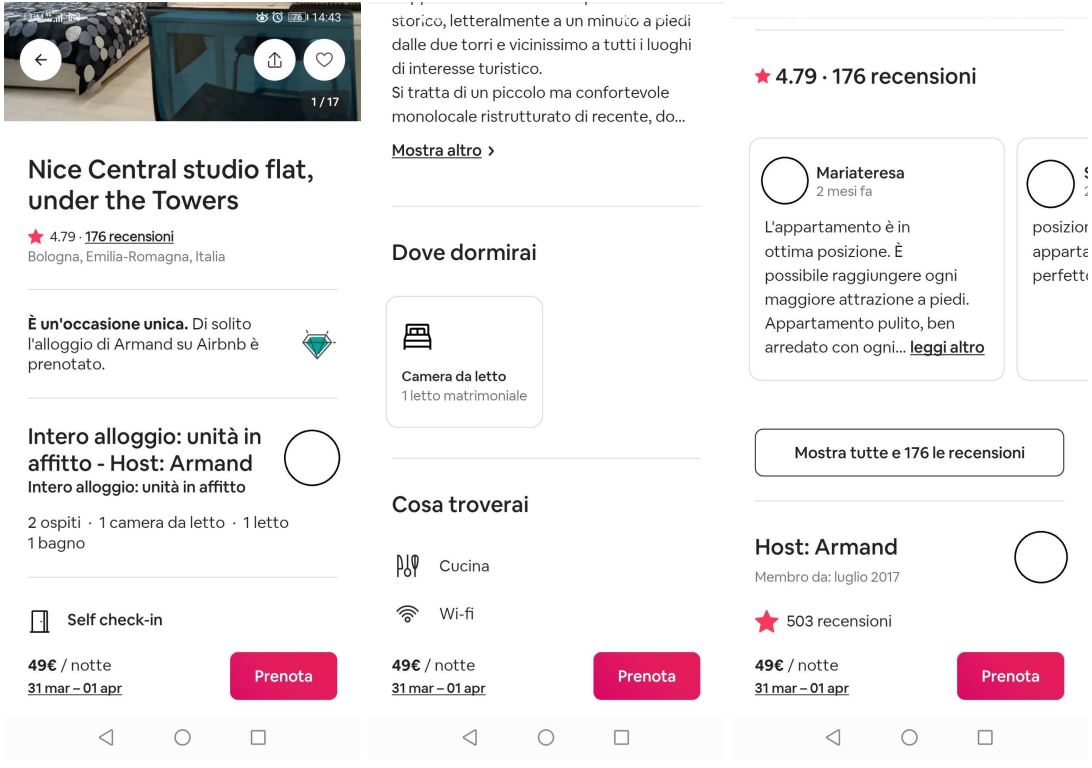
\includegraphics{resources/airbnb.png}
\newline
Al termine del soggiorno, gli ospiti e gli host si possono valutare a vicenda. La recensione
fatta dagli ospiti comprende due testi (uno per l’appartamento e uno per l’host) e una serie di
punteggi in una scala da 1 a 5 su dimensioni come pulizia, comunicazione, posizione,
qualità/prezzo. La valutazione complessiva del soggiorno è una media delle valutazioni
ricevute sulle singole dimensioni. Le recensioni degli host comprendono solo un commento
testuale. Le recensioni possono essere visibili o non visibili. Diventano visibili quando
entrambi hanno fatto la recensione oppure se uno dei due non ha fatto la recensione, l’altra
diventa visibile dopo 7 giorni dalla fine del soggiorno. Gli host e gli ospiti possono
commentare più volte le review in cui sono coinvolti, creando un thread di discussione.
Le recensioni sono visibili sui profili degli utenti suddivise in base a quelle ricevute come
ospite e come host. La base di dati deve supportare le seguenti operazioni:
\begin{itemize}
    \item Una volta a settimana viene effettuato un calcolo per aggiornare il tasso di
    cancellazione di ciascun host.
    \item Una volta al giorno si controllano le condizioni per la qualifica di superhost e viene
    aggiornato lo status degli host.
    \item Una volta al mese viene calcolata la classifica degli alloggi più graditi.
\end{itemize}
